\chapter{Resultados}
\label{chap:resultados}

\section{Temperatura e Umidade}
\label{chap:temperatura-umidade}

oi
        \begin{figure}[!h]
		\Caption{\label{fig:figura-temperatura-variaveis} Variáveis utilizadas para o projeto.}
		%\centering
		\UFCfig{}{
			\fbox{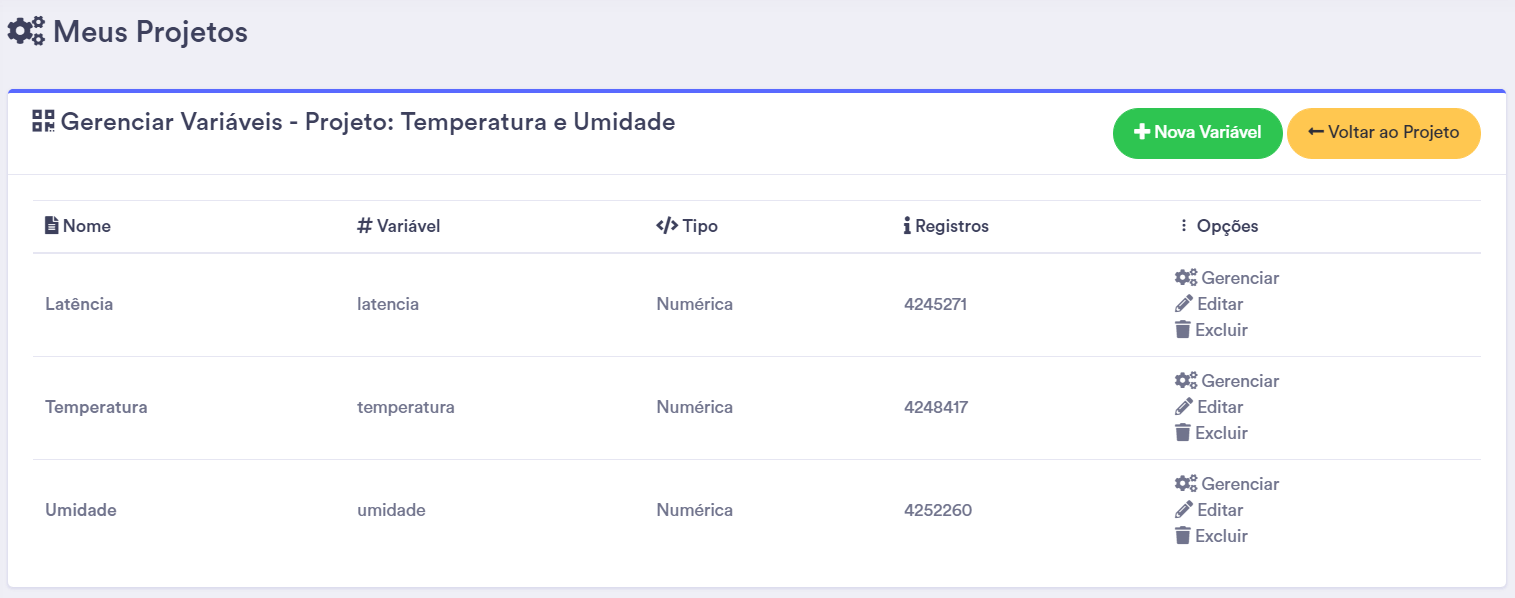
\includegraphics[width=15cm]{figuras/temperatura-variaveis.png}}
		}{
			\Fonte{O autor}
		}	
    	\end{figure}
    	
oi
        \begin{figure}[!h]
		\Caption{\label{fig:figura-temperatura-instataneos} Últimas informações enviadas.}
		%\centering
		\UFCfig{}{
			\fbox{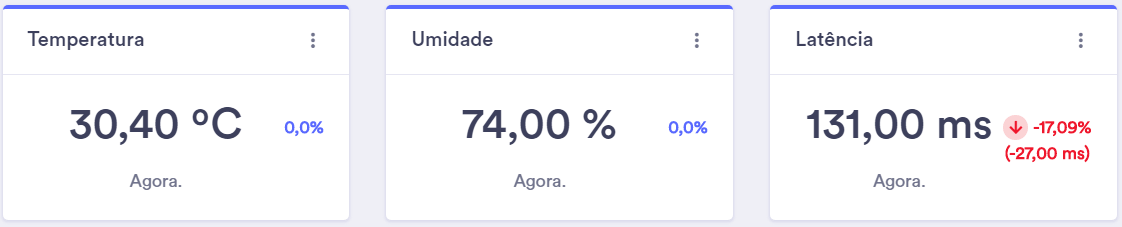
\includegraphics[width=15cm]{figuras/temperatura-instataneos.png}}
		}{
			\Fonte{O autor}
		}	
    	\end{figure}
    	
oi
        \begin{figure}[!h]
		\Caption{\label{fig:figura-temperatura-grafico} Gráfico de área com os últimos 30 minutos de temperatura registrada.}
		%\centering
		\UFCfig{}{
			\fbox{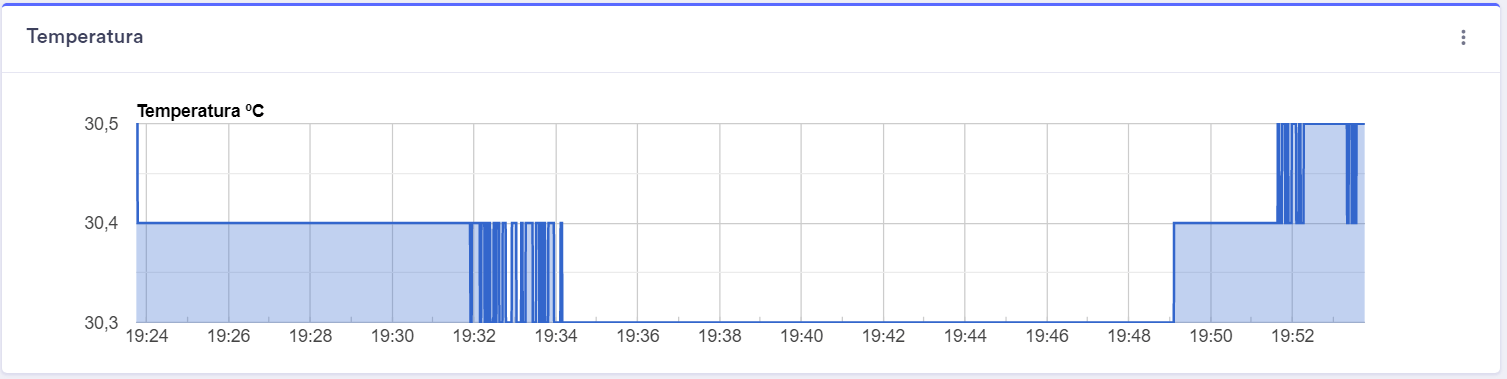
\includegraphics[width=15cm]{figuras/temperatura-grafico.png}}
		}{
			\Fonte{O autor}
		}	
    	\end{figure}

oi
        \begin{figure}[!h]
		\Caption{\label{fig:figura-temperatura-umidade} Gráfico de área com os últimos 30 minutos de umidade registrada.}
		%\centering
		\UFCfig{}{
			\fbox{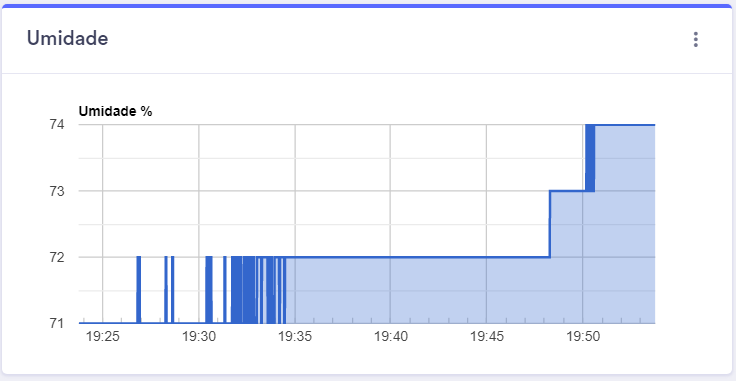
\includegraphics[width=15cm]{figuras/temperatura-umidade.png}}
		}{
			\Fonte{O autor}
		}	
    	\end{figure}
    	
oi
        \begin{figure}[!h]
		\Caption{\label{fig:figura-temperatura-latencia} Gráfico de linhas com os últimos 30 minutos de latência registrada.}
		%\centering
		\UFCfig{}{
			\fbox{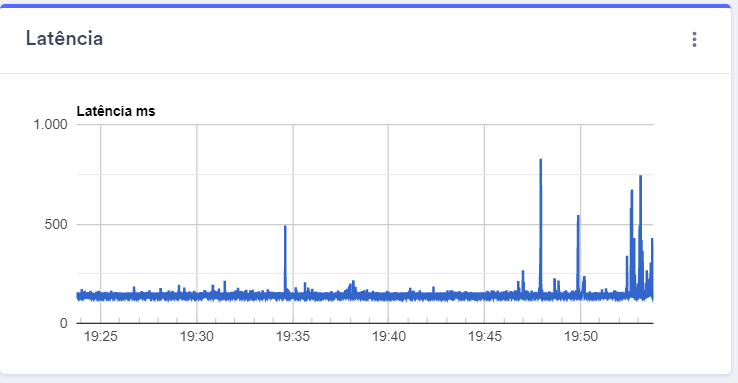
\includegraphics[width=15cm]{figuras/temperatura-latencia.png}}
		}{
			\Fonte{O autor}
		}	
    	\end{figure}
\section{Qualidade Sinal - WiFi}
\label{chap:qualidade-sinal}
oi

        \begin{figure}[!h]
		\Caption{\label{fig:figura-wifi-variaveis} Variáveis utilizadas no projeto.}
		%\centering
		\UFCfig{}{
			\fbox{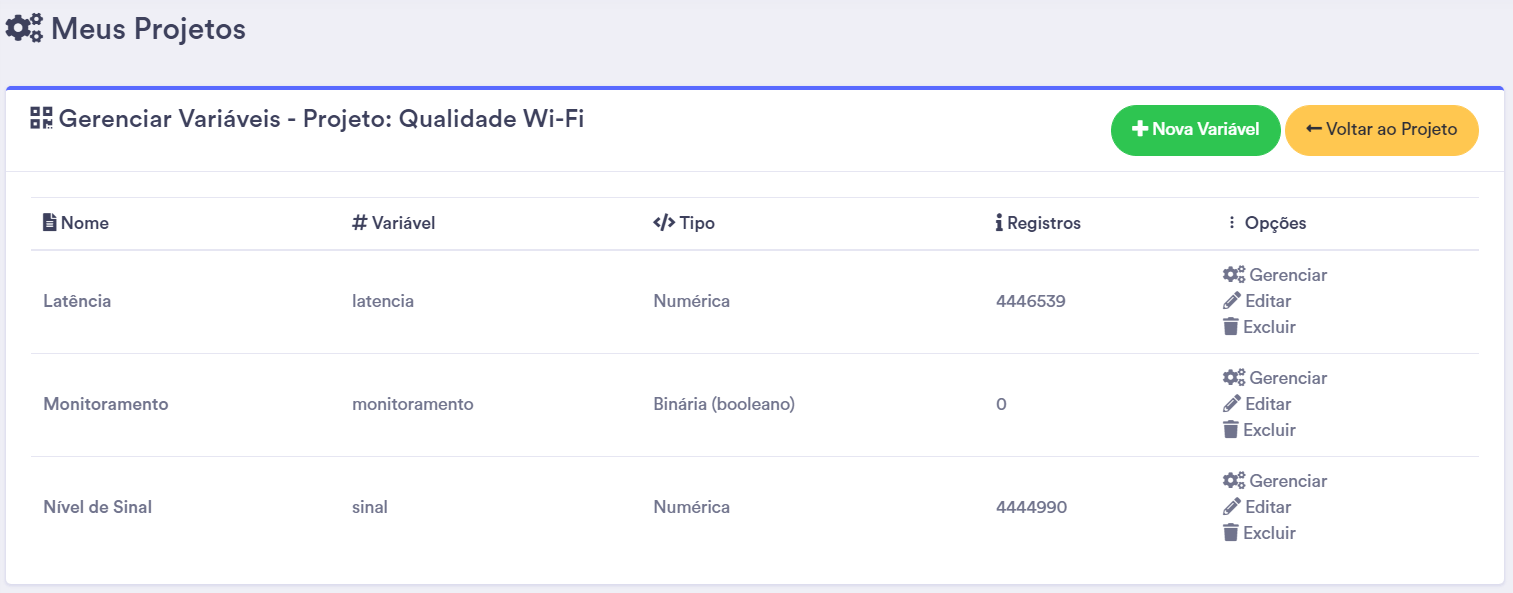
\includegraphics[width=15cm]{figuras/wifi-variaveis.png}}
		}{
			\Fonte{O autor}
		}	
    	\end{figure}
    	
oi

        \begin{figure}[!h]
		\Caption{\label{fig:figura-wifi-instataneos} Botão para ação no processo além de últimas informações enviadas.}
		%\centering
		\UFCfig{}{
			\fbox{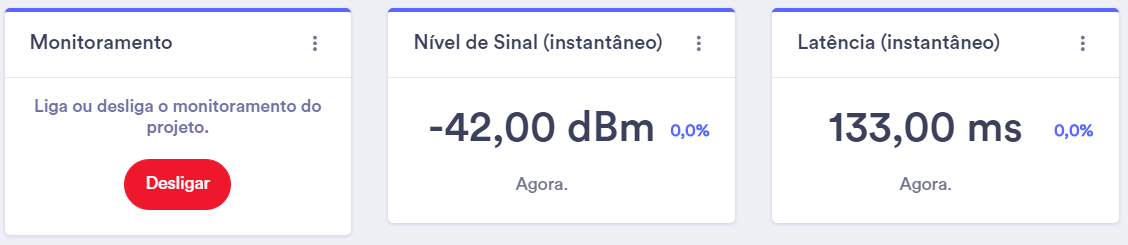
\includegraphics[width=15cm]{figuras/wifi-instataneos.png}}
		}{
			\Fonte{O autor}
		}	
    	\end{figure}
    	
oi

        \begin{figure}[!h]
		\Caption{\label{fig:figura-wifi-sinal} Gráfico de linhas com os últimos 30 minutos de qualidade de sinal registrada.}
		%\centering
		\UFCfig{}{
			\fbox{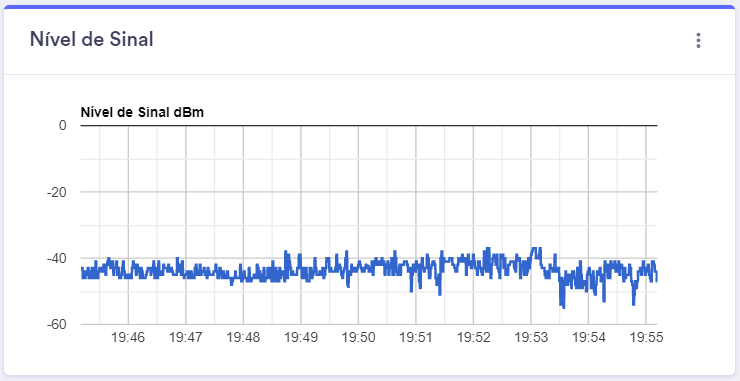
\includegraphics[width=15cm]{figuras/wifi-sinal.png}}
		}{
			\Fonte{O autor}
		}	
    	\end{figure}
    	
oi

        \begin{figure}[!h]
		\Caption{\label{fig:figura-wifi-latencia} Gráfico de linhas com os últimos 10 minutos de latência registrada.}
		%\centering
		\UFCfig{}{
			\fbox{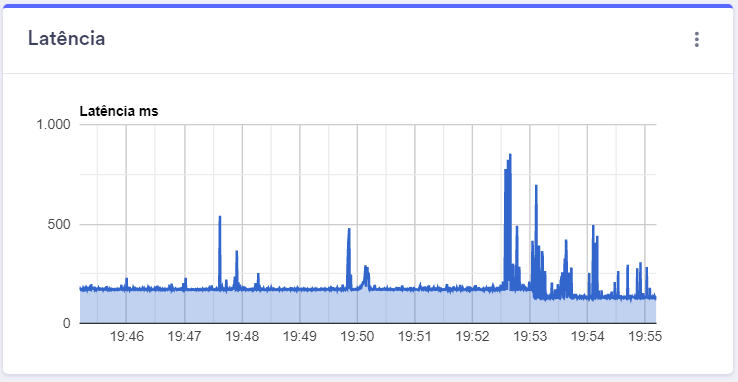
\includegraphics[width=15cm]{figuras/wifi-latencia.png}}
		}{
			\Fonte{O autor}
		}	
    	\end{figure}
    	


\section{Demanda de Roteadores}
\label{chap:demanda-roteadores}
oi

        \begin{figure}[!h]
		\Caption{\label{fig:figura-roteadores-recepcao} Quantidade de hóspedes conectados no roteador da recepção durante 24 horas.}
		%\centering
		\UFCfig{}{
			\fbox{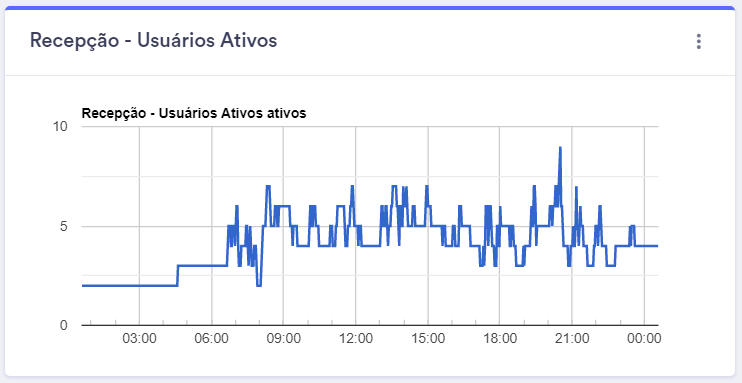
\includegraphics[width=15cm]{figuras/roteadores-recepcao.png}}
		}{
			\Fonte{O autor}
		}	
    	\end{figure}
    	
oi

        \begin{figure}[!h]
		\Caption{\label{fig:figura-roteadores-recepcao-downlink} Uso máximo de downlink pelo roteador da recepção durante 24 horas.}
		%\centering
		\UFCfig{}{
			\fbox{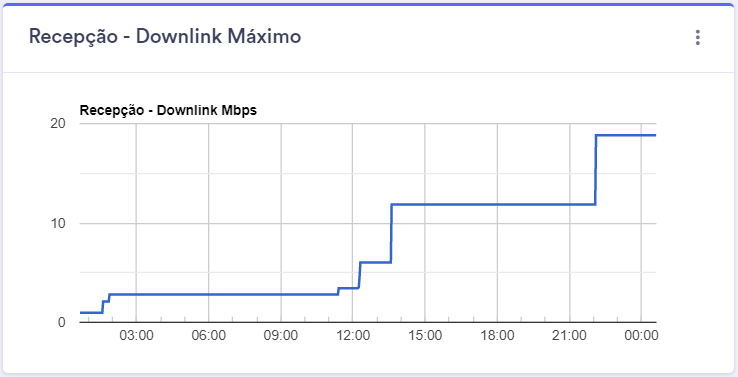
\includegraphics[width=15cm]{figuras/roteadores-recepcao-downlink.png}}
		}{
			\Fonte{O autor}
		}	
    	\end{figure}
    	
oi

        \begin{figure}[!h]
		\Caption{\label{fig:figura-roteadores-107} Quantidade de hóspedes conectados no roteador "107" durante 24 horas.}
		%\centering
		\UFCfig{}{
			\fbox{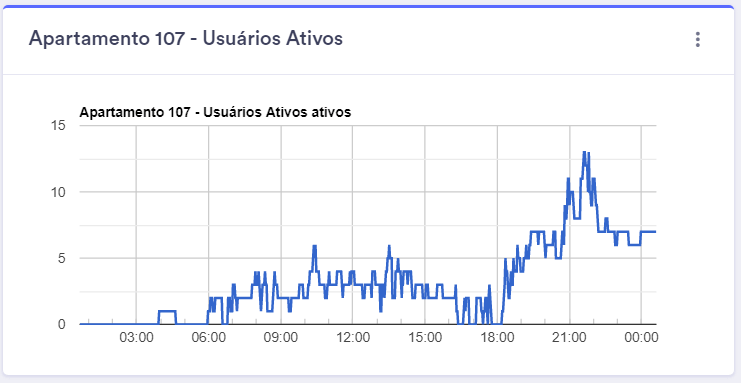
\includegraphics[width=15cm]{figuras/roteadores-107.png}}
		}{
			\Fonte{O autor}
		}	
    	\end{figure}
    	
oi

        \begin{figure}[!h]
		\Caption{\label{fig:figura-roteadores-107-downlink} Uso máximo de downlink pelo roteador "107" durante 24 horas.}
		%\centering
		\UFCfig{}{
			\fbox{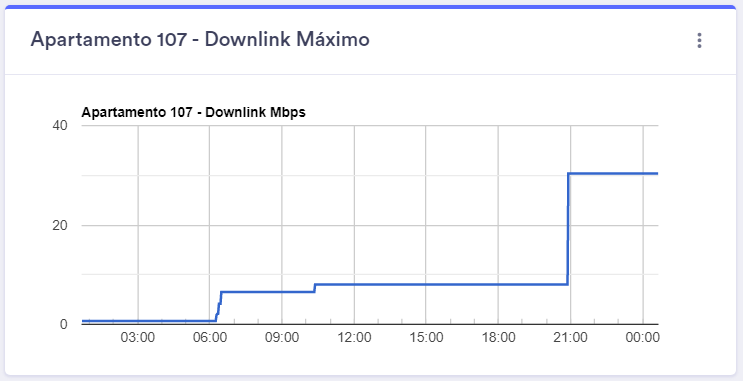
\includegraphics[width=15cm]{figuras/roteadores-107-downlink.png}}
		}{
			\Fonte{O autor}
		}	
    	\end{figure}